\documentclass[tikz,border=10px, convert={density=300,outext=.png}]{standalone}
\usepackage{tikz}
\usetikzlibrary{shapes.geometric, arrows, positioning, fit, calc, backgrounds}

\begin{document}

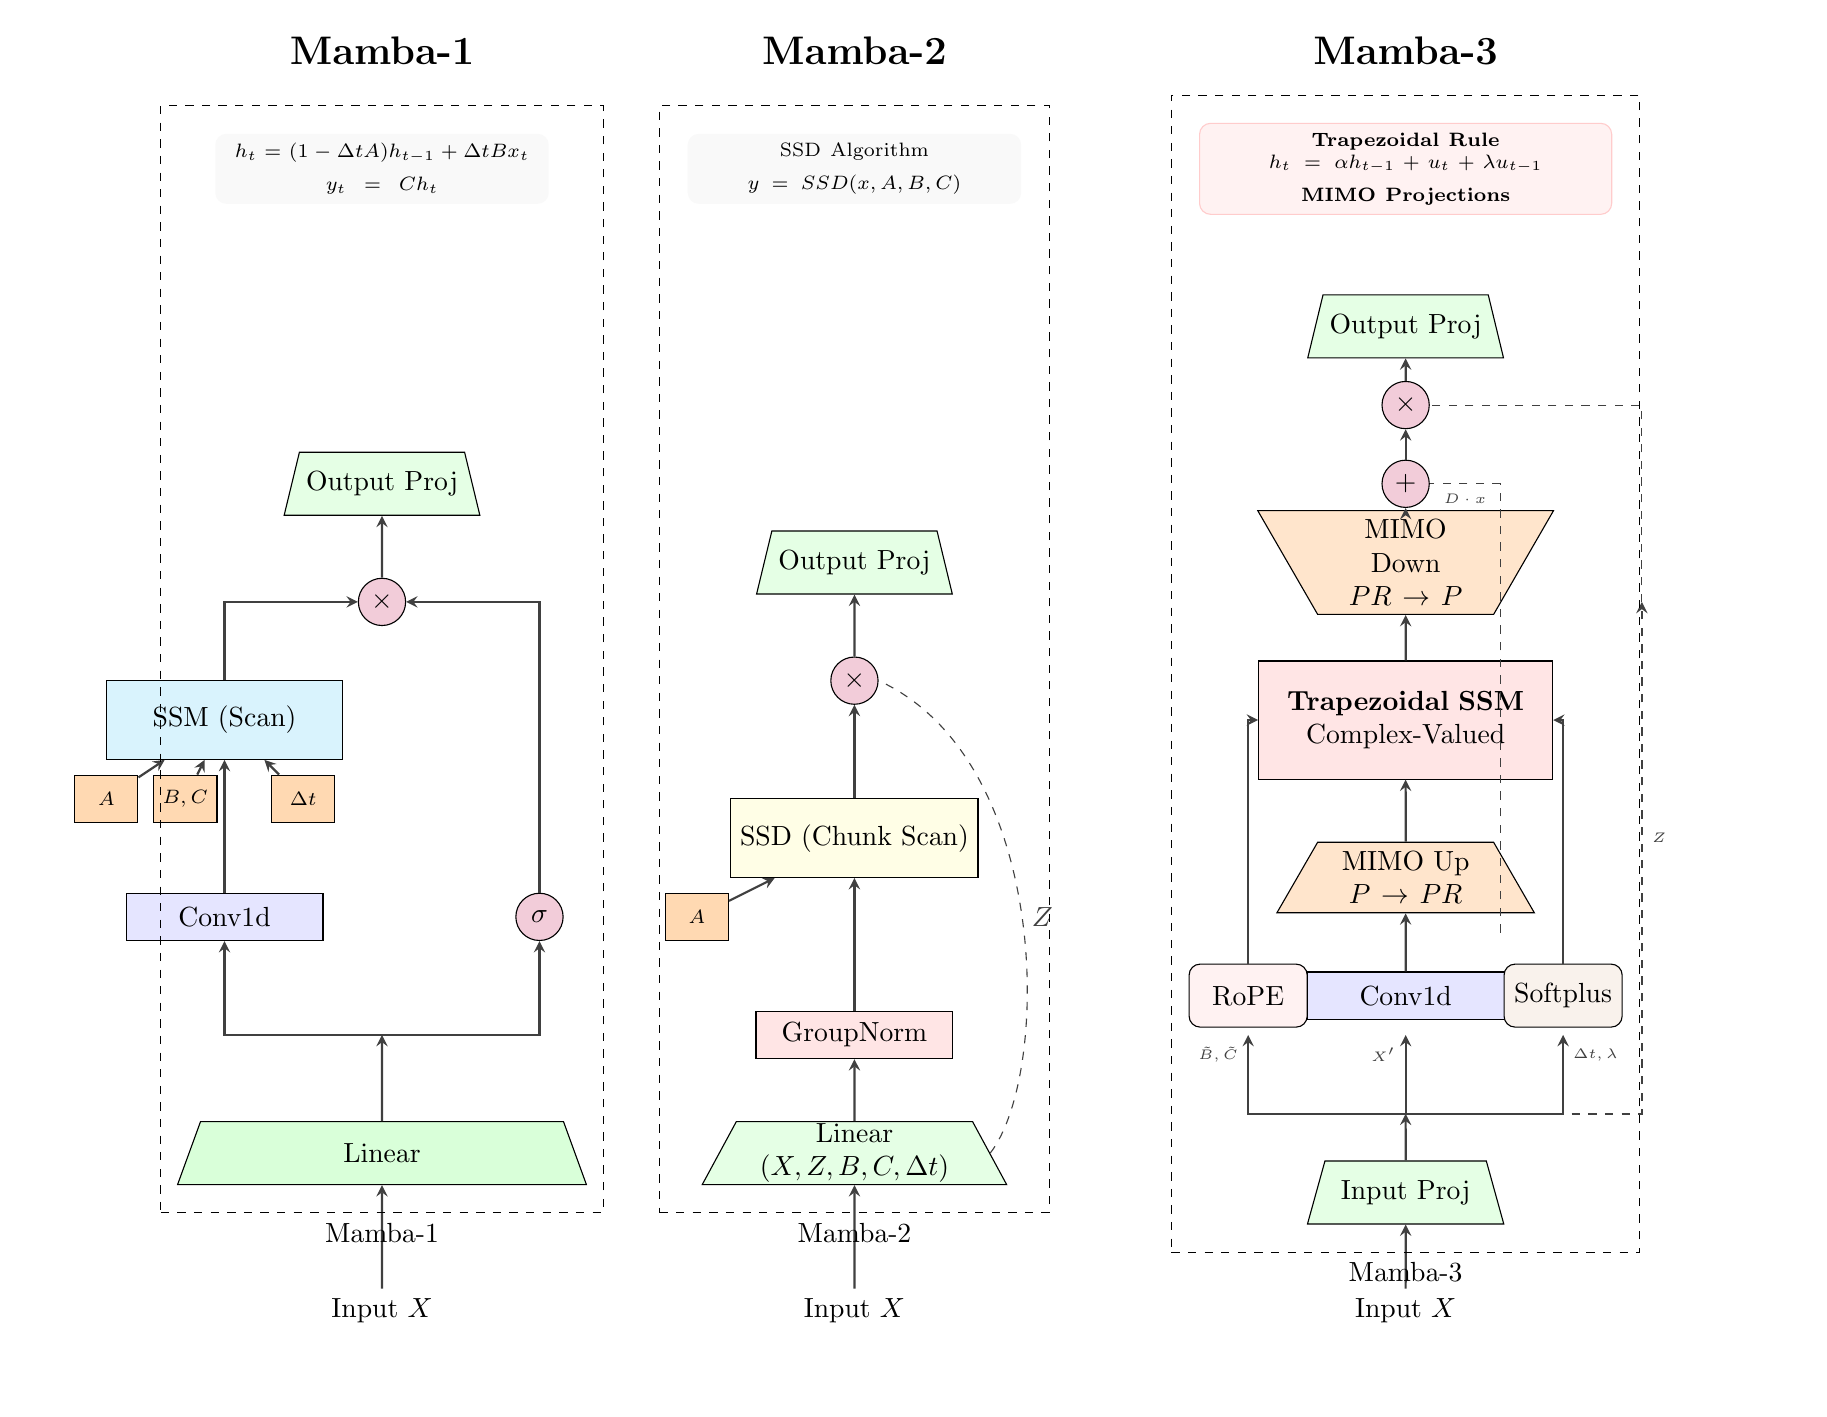
\begin{tikzpicture}[
    node distance=1.0cm,
    block/.style={trapezium, trapezium stretches=true, draw, fill=green!10, minimum width=2.5cm, minimum height=0.8cm, text centered, inner sep=0pt},
    rect/.style={rectangle, draw, rounded corners, fill=blue!10, minimum width=2.5cm, minimum height=0.8cm, text centered},
    param/.style={rectangle, draw, fill=orange!30, minimum width=0.8cm, minimum height=0.6cm, text centered, font=\scriptsize},
    op/.style={circle, draw, fill=purple!20, minimum size=0.6cm, inner sep=0pt, text centered},
    conn/.style={->, >=stealth, thick, darkgray}
]

% White Background
\path [fill=white] (-4.5, -1) rectangle (18, 16);

% Define styles
\tikzstyle{projection} = [trapezium, trapezium left angle=70, trapezium right angle=70, draw, fill=green!15, text width=2.5cm, align=center, minimum height=0.8cm]
\tikzstyle{ssm} = [rectangle, draw, fill=cyan!15, minimum width=3cm, minimum height=1cm, align=center]
\tikzstyle{conv} = [rectangle, draw, fill=blue!10, minimum width=2.5cm, minimum height=0.6cm, align=center]
\tikzstyle{norm} = [rectangle, draw, fill=red!10, minimum width=2.5cm, minimum height=0.6cm, align=center]
\tikzstyle{gate} = [circle, draw, fill=white, inner sep=1pt]
\tikzstyle{dot} = [circle, fill, inner sep=1.5pt]

% ==================== MAMBA 1 ====================
\node[font=\bfseries\Large] (title1) at (0, 16) {Mamba-1};

\node[text width=4cm, align=center, fill=gray!5, rounded corners] (formula1) at (0, 14.5) {
    \scriptsize $h_t = (1-\Delta t A)h_{t-1} + \Delta t B x_t$\\
    \scriptsize $y_t = C h_t$
};

\node (in1) at (0, 0) {Input $X$};
\node[projection] (proj1) at (0, 2) {Linear};
\draw[conn] (in1) -- (proj1);

% Split
\coordinate (split1) at (0, 3.5);
\draw[conn] (proj1) -- (split1);

% Left Branch (Main)
\node[conv] (conv1) at (-2, 5) {Conv1d};
\draw[conn] (split1) -| (conv1);

\node[ssm] (ssm1) at (-2, 7.5) {SSM (Scan)};
\draw[conn] (conv1) -- (ssm1);

% Parameters
\node[param] (A1) at (-3.5, 6.5) {$A$};
\node[param] (B1) at (-2.5, 6.5) {$B, C$};
\draw[conn] (A1) -- (ssm1);
\draw[conn] (B1) -- (ssm1);
\node[param] (dt1) at (-1, 6.5) {$\Delta t$};
\draw[conn] (dt1) -- (ssm1);

% Right Branch (Gate)
\node[op] (silu1) at (2, 5) {$\sigma$};
\draw[conn] (split1) -| (silu1);

% Merge
\node[op] (mult1) at (0, 9) {$\times$};
\draw[conn] (ssm1.north) |- (mult1);
\draw[conn] (silu1.north) |- (mult1);

\node[block] (out1_rect) at (0, 10.5) {Output Proj};
\draw[conn] (mult1) -- (out1_rect);

% ==================== MAMBA 2 ====================
\node[font=\bfseries\Large] (title2) at (6, 16) {Mamba-2};

\node[text width=4cm, align=center, fill=gray!5, rounded corners] (formula2) at (6, 14.5) {
    \scriptsize SSD Algorithm\\
    \scriptsize $y = \text{SSD}(x, A, B, C)$
};

\node (in2) at (6, 0) {Input $X$};
\node[block, text width=3cm] (proj2) at (6, 2) {Linear ($X, Z, B, C, \Delta t$)};
\draw[conn] (in2) -- (proj2);

% Norm
\node[norm] (norm2) at (6, 3.5) {GroupNorm};
\draw[conn] (proj2) -- (norm2);

% SSD
\node[ssm, fill=yellow!10] (ssd2) at (6, 6) {SSD (Chunk Scan)};
\draw[conn] (norm2) -- (ssd2);

% Parameters feed
\node[param] (A2) at (4, 5) {$A$};
\draw[conn] (A2) -- (ssd2);

% Gate (Z)
\coordinate (split2) at (6, 3);
\node[op] (mult2) at (6, 8) {$\times$};
\draw[conn] (ssd2) -- (mult2);

% Z path
\draw[dashed, darkgray] (proj2.east) .. controls (8.5, 3) and (8.5, 7) .. (mult2.east) node[midway, right] {$Z$};

\node[block] (out2) at (6, 9.5) {Output Proj};
\draw[conn] (mult2) -- (out2);


% ==================== MAMBA 3 ====================
\node[font=\bfseries\Large] (title3) at (13, 16) {Mamba-3};

\node[text width=5cm, align=center, fill=red!5, rounded corners, draw=red!20] (formula3) at (13, 14.5) {
    \scriptsize \textbf{Trapezoidal Rule}\\
    \scriptsize $h_t = \alpha h_{t-1} + u_t + \lambda u_{t-1}$\\
    \scriptsize \textbf{MIMO Projections}
};

\node (in3) at (13, 0) {Input $X$};
\node[block] (proj3) at (13, 1.5) {Input Proj};
\draw[conn] (in3) -- (proj3);

% Split
\coordinate (split3) at (13, 2.5);
\draw[conn] (proj3) -- (split3);

% Branches
\node (b_x) at (13, 3) {};
\node (b_bc) at (11, 3) {};
\node (b_dt) at (15, 3) {};
\node (b_z) at (16, 3) {};

\draw[conn] (split3) -- (b_x.center) -- node[left, font=\tiny] {$X'$} ++(0, 0.5);
\draw[conn] (split3) -| (b_bc.center) -- node[left, font=\tiny] {$\tilde{B}, \tilde{C}$} ++(0, 0.5);
\draw[conn] (split3) -| (b_dt.center) -- node[right, font=\tiny] {$\Delta t, \lambda$} ++(0, 0.5);
\draw[conn, dashed] (split3) -| (b_z.center) -- node[right, font=\tiny] {$Z$} ++(0, 6); % Z path

% Components
\node[conv] (conv3) at (13, 4) {Conv1d};
\node[rect, fill=pink!20, minimum width=1.5cm] (rope3) at (11, 4) {RoPE};
\node[rect, fill=brown!10, minimum width=1.5cm] (soft3) at (15, 4) {Softplus};

% MIMO Up
\node[trapezium, draw, fill=orange!20, minimum width=2.5cm, text width=2cm, align=center] (mimo_up) at (13, 5.5) {MIMO Up\\$P \to PR$};
\draw[conn] (conv3) -- (mimo_up);

% SSM
\node[ssm, fill=red!10, text width=3.5cm, minimum height=1.5cm] (trap3) at (13, 7.5) {\textbf{Trapezoidal SSM}\\Complex-Valued};

% Connections to SSM
\draw[conn] (mimo_up) -- (trap3);
\draw[conn] (rope3) |- (trap3.west);
\draw[conn] (soft3) |- (trap3.east);

% MIMO Down
\node[trapezium, shape border rotate=180, draw, fill=orange!20, minimum width=2.5cm, text width=2cm, align=center] (mimo_down) at (13, 9.5) {MIMO Down\\$PR \to P$};
\draw[conn] (trap3) -- (mimo_down);

% Skip connection
\node[op] (add3) at (13, 10.5) {$+$};
\draw[conn] (mimo_down) -- (add3);
\draw[dashed, darkgray] (14.2, 4.8) -- (14.2, 10.5) -- (add3) node[midway, below] {\tiny $D \cdot x$};

% Gate
\node[op] (mult3) at (13, 11.5) {$\times$};
\draw[conn] (add3) -- (mult3);
\draw[dashed, darkgray] (16, 9) -- (16, 11.5) -- (mult3); % Z ends here

\node[block] (out3) at (13, 12.5) {Output Proj};
\draw[conn] (mult3) -- (out3);

% Boxes around
\node[draw, dashed, inner sep=10pt, fit=(proj1) (out1_rect) (formula1), label=below:Mamba-1] {};
\node[draw, dashed, inner sep=10pt, fit=(proj2) (out2) (formula2), label=below:Mamba-2] {};
\node[draw, dashed, inner sep=10pt, fit=(proj3) (out3) (formula3), label=below:Mamba-3] {};

\end{tikzpicture}

\end{document}
